\chapter{Appendix}

\printglossaries

\newpage


\section{IterationLogger Fields}
\label{des:iterationdatafields}

The following fields are currently available in the IterationData file. The IterationData file is a CSV file containing the configuration and performance data for each iteration of the simulation. The data is collected and logged by the \texttt{IterationLogger} class of the \gls{autopas} library.

\begin{description}[style=multiline, leftmargin =40mm]
  \item[Date] The date and time when the data was collected.
  \item[Iteration] The current iteration number of the simulation.
  \item[inTuningPhase] Indicates whether the simulation is in the tuning phase (true/false).
  \item[Container] The type of container used to store the particles in the simulation (e.g., LinkedCells, VerletLists).
  \item[CellSizeFactor] A factor that determines the size of the cells relative to the cutoff radius.
  \item[Traversal] The method used to traverse the cells and calculate interactions between particles.
  \item[Load Estimator] The strategy used to estimate and balance the computational load across different parts of the simulation domain.
  \item[Data Layout] The arrangement of particle data in memory (e.g., AoS for Array of Structures, SoA for Structure of Arrays).
  \item[Newton 3] Indicates whether Newton's third law optimization is used to reduce computation by only calculating forces once per particle pair (enabled/disabled).
  \item[iteratePairwise] The time taken to iterate over all particle pairs and calculate interactions.
  \item[remainderTraversal] The time taken to perform any remaining traversal operations.
  \item[rebuildNeighborLists] The time taken to rebuild the neighbor lists.
  \item[iteratePairwiseTotal] The total time taken to iterate over all particle pairs and calculate interactions.
  \item[tuning] The time taken to perform any tuning operations.
  \item[energyPsys] The energy consumed by the system (in Joules).
  \item[energyPkg] The energy consumed by the package (CPU) (in Joules).
  \item[energyRam] The energy consumed by the RAM (in Joules).
\end{description}


\section{TuningDataLogger Fields}
\label{des:tuningdatafields}

The following fields are currently available in the TuningData file.
The TuningData file is a CSV file containing the performance information for all tested configurations. The data is collected and logged by the \texttt{TuningDataLogger} class of the \gls{autopas} library.

\begin{description}[style=multiline, leftmargin =40mm]
  \item[Date] The date and time when the data was collected.
  \item[Iteration] The current iteration number of the simulation.
  \item[Container] The type of container used to store the particles in the simulation (e.g., LinkedCells, VerletLists).
  \item[CellSizeFactor] A factor that determines the size of the cells relative to the cutoff radius.
  \item[Traversal] The method used to traverse the cells and calculate interactions between particles.
  \item[Load Estimator] The strategy used to estimate and balance the computational load across different parts of the simulation domain.
  \item[Data Layout] The arrangement of particle data in memory (e.g., AoS for Array of Structures, SoA for Structure of Arrays).
  \item[Newton 3] Indicates whether Newton's third law optimization is used to reduce computation by only calculating forces once per particle pair (enabled/disabled).
  \item[Reduced] The reduced performance data for all sample points is calculated by aggregating the data across all sample points. The specific aggregation method can be configured via the \texttt{.yaml} configuration file.
  \item[Smoothed] A smoothed version of the reduced performance data.

\end{description}

\section{LiveInfoLogger Fields}
\label{des:liveinfodatafields}

The following fields are currently available in the LiveInfoData file. The LiveInfoData file is a CSV file containing summary statistics about the simulation state at each iteration. The data is collected and logged by the \texttt{LiveInfoLogger} class of the \gls{autopas} library.

\begin{description}[style=multiline, leftmargin =40mm]
  \item [Iteration] The current iteration number of the simulation.
  \item [avgParticlesPerCell] The average number of particles per cell in the simulation domain.
  \item [cutoff] The cutoff radius for the interaction of particles, beyond which particles do not interact.
  \item [domainSizeX] The size of the simulation domain in the X dimension.
  \item [domainSizeY] The size of the simulation domain in the Y dimension.
  \item [domainSizeZ] The size of the simulation domain in the Z dimension.
  \item [estimatedNumNeighborInteractions] The estimated number of neighbor interactions between all particles in the simulation domain.
  \item [homogeneity] A measure of the distribution uniformity of particles across the cells.
  \item [maxDensity] The maximum density of particles in any cell.
  \item [maxParticlesPerCell] The maximum number of particles found in any single cell.
  \item [minParticlesPerCell] The minimum number of particles found in any single cell.
  \item [numCells] The total number of cells in the simulation domain.
  \item [numEmptyCells] The number of cells that contain no particles.
  \item [numHaloParticles] The number of particles in the halo region (boundary region) of the simulation domain.
  \item [numParticles] The total number of particles in the simulation domain.
  \item [particleSize] The number of bytes used to store a single particle in memory.
  \item [particleSizeNeededByFunctor] The particle size required by the functor (the function used for calculating interactions).
  \item [particlesPerBlurredCellStdDev] The standard deviation of the number of particles per blurred cell provides a measure of particle distribution variability.
  \item [particlesPerCellStdDev] The standard deviation of the number of particles per cell, indicating the variability in particle distribution.
  \item [rebuildFrequency] The frequency at which the neighbor list is rebuilt.
  \item [skin] The skin width is added to the cutoff radius to create a buffer zone for neighbor lists, ensuring efficient interaction calculations.
  \item [threadCount] The number of threads used for parallel processing in the simulation.
\end{description}



\section{Scenarios used for Data Generation}
\label{des:scenarios}

The scenarios used for data generation stem directly from the examples provided in the \texttt{AutoPas} library. Their state at the time of the data generation can be looked up at \small{
  \url{
    https://github.com/AutoPas/AutoPas/tree/563528b4ef55d29b8ec148f6387f0be1adb400ed/examples/md-flexible/input
  }
}

The specific scenarios used are: \texttt{explodingLiquid}, \texttt{spinodalDecompositionEquilibration}, \texttt{spinodalDecomposition}, and \texttt{fallingDrop}.


\section{Data Analysis}

We performed some exploratory data analysis to gain insights into the collected dataset. The results are presented in the following figures.

\begin{figure}[H]
  \centering
  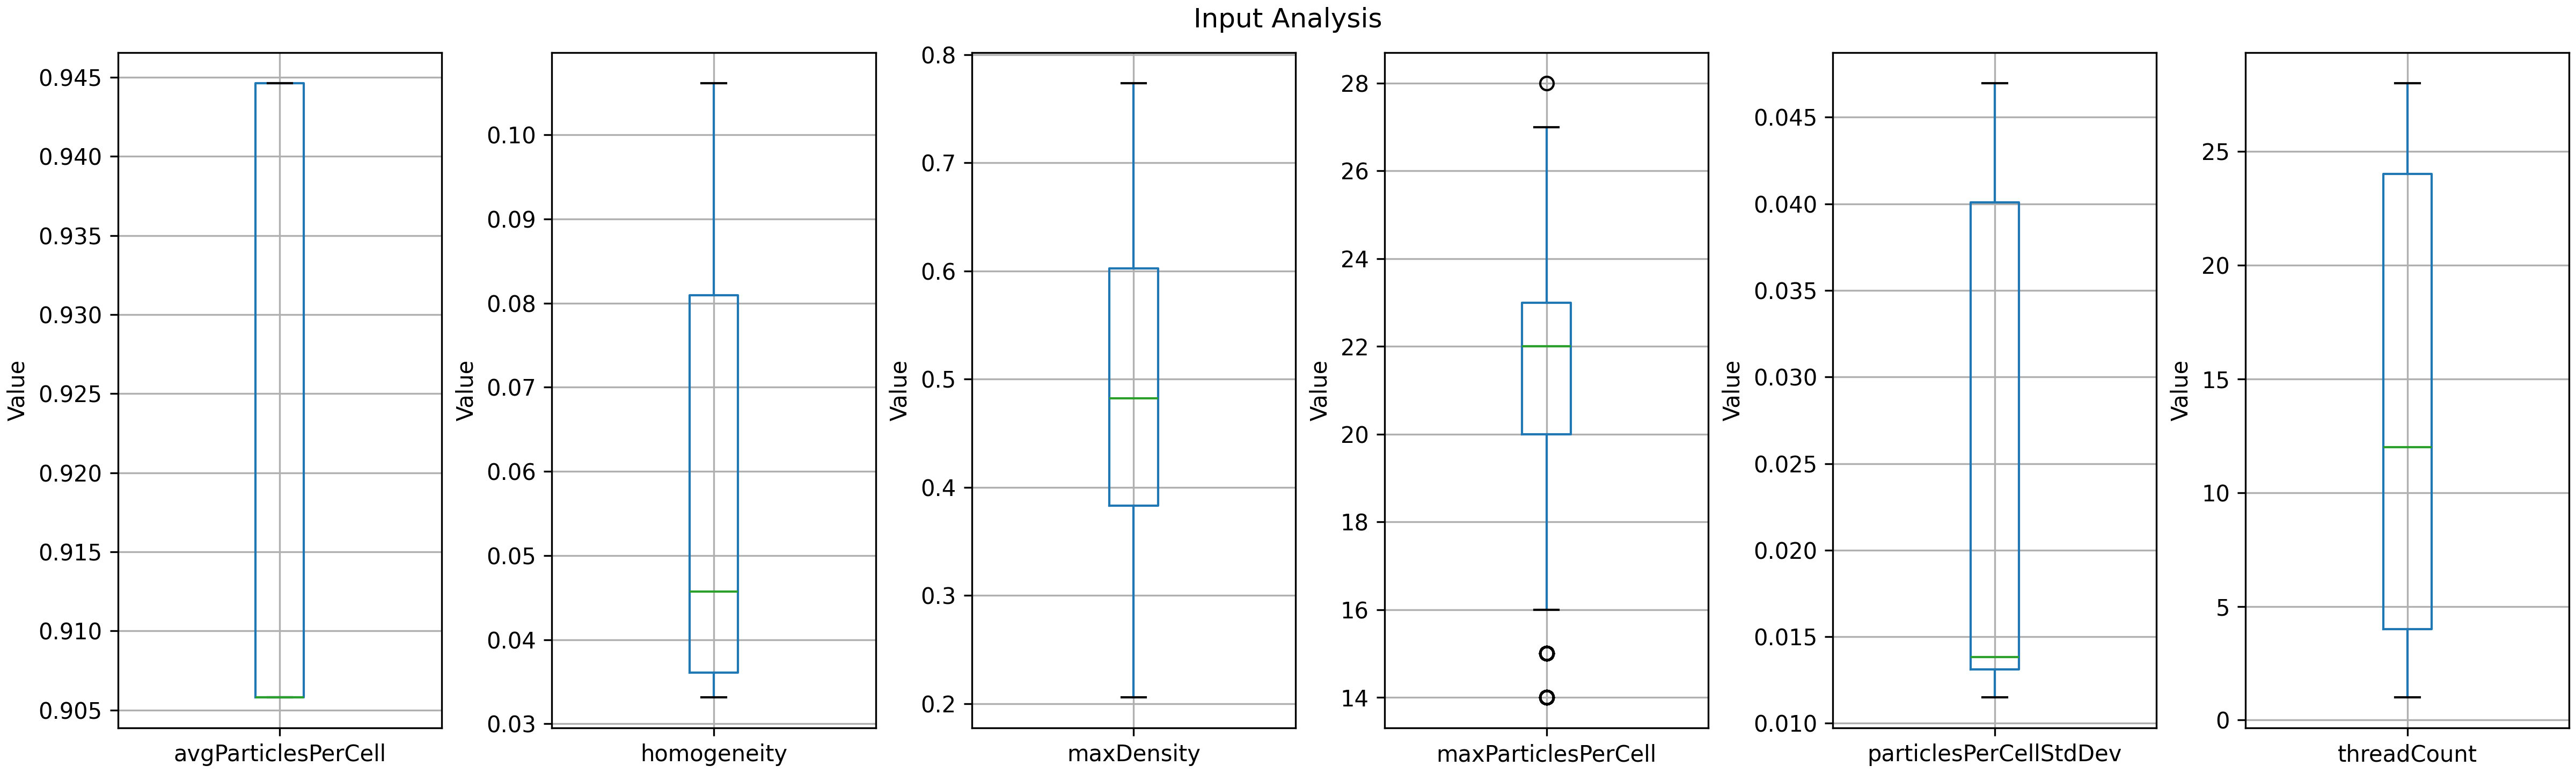
\includegraphics[width=\columnwidth,trim={0 0 0 0.5cm},clip]{figures/DataAnalytics/input_analysis.png}
  \caption[Boxplot of the collected Dataset]{Boxplot showing the distribution of the collected data of the LiveInfoData files}
  \label{fig:inputAnalysisBoxplot}
\end{figure}

\begin{figure}[H]
  \centering
  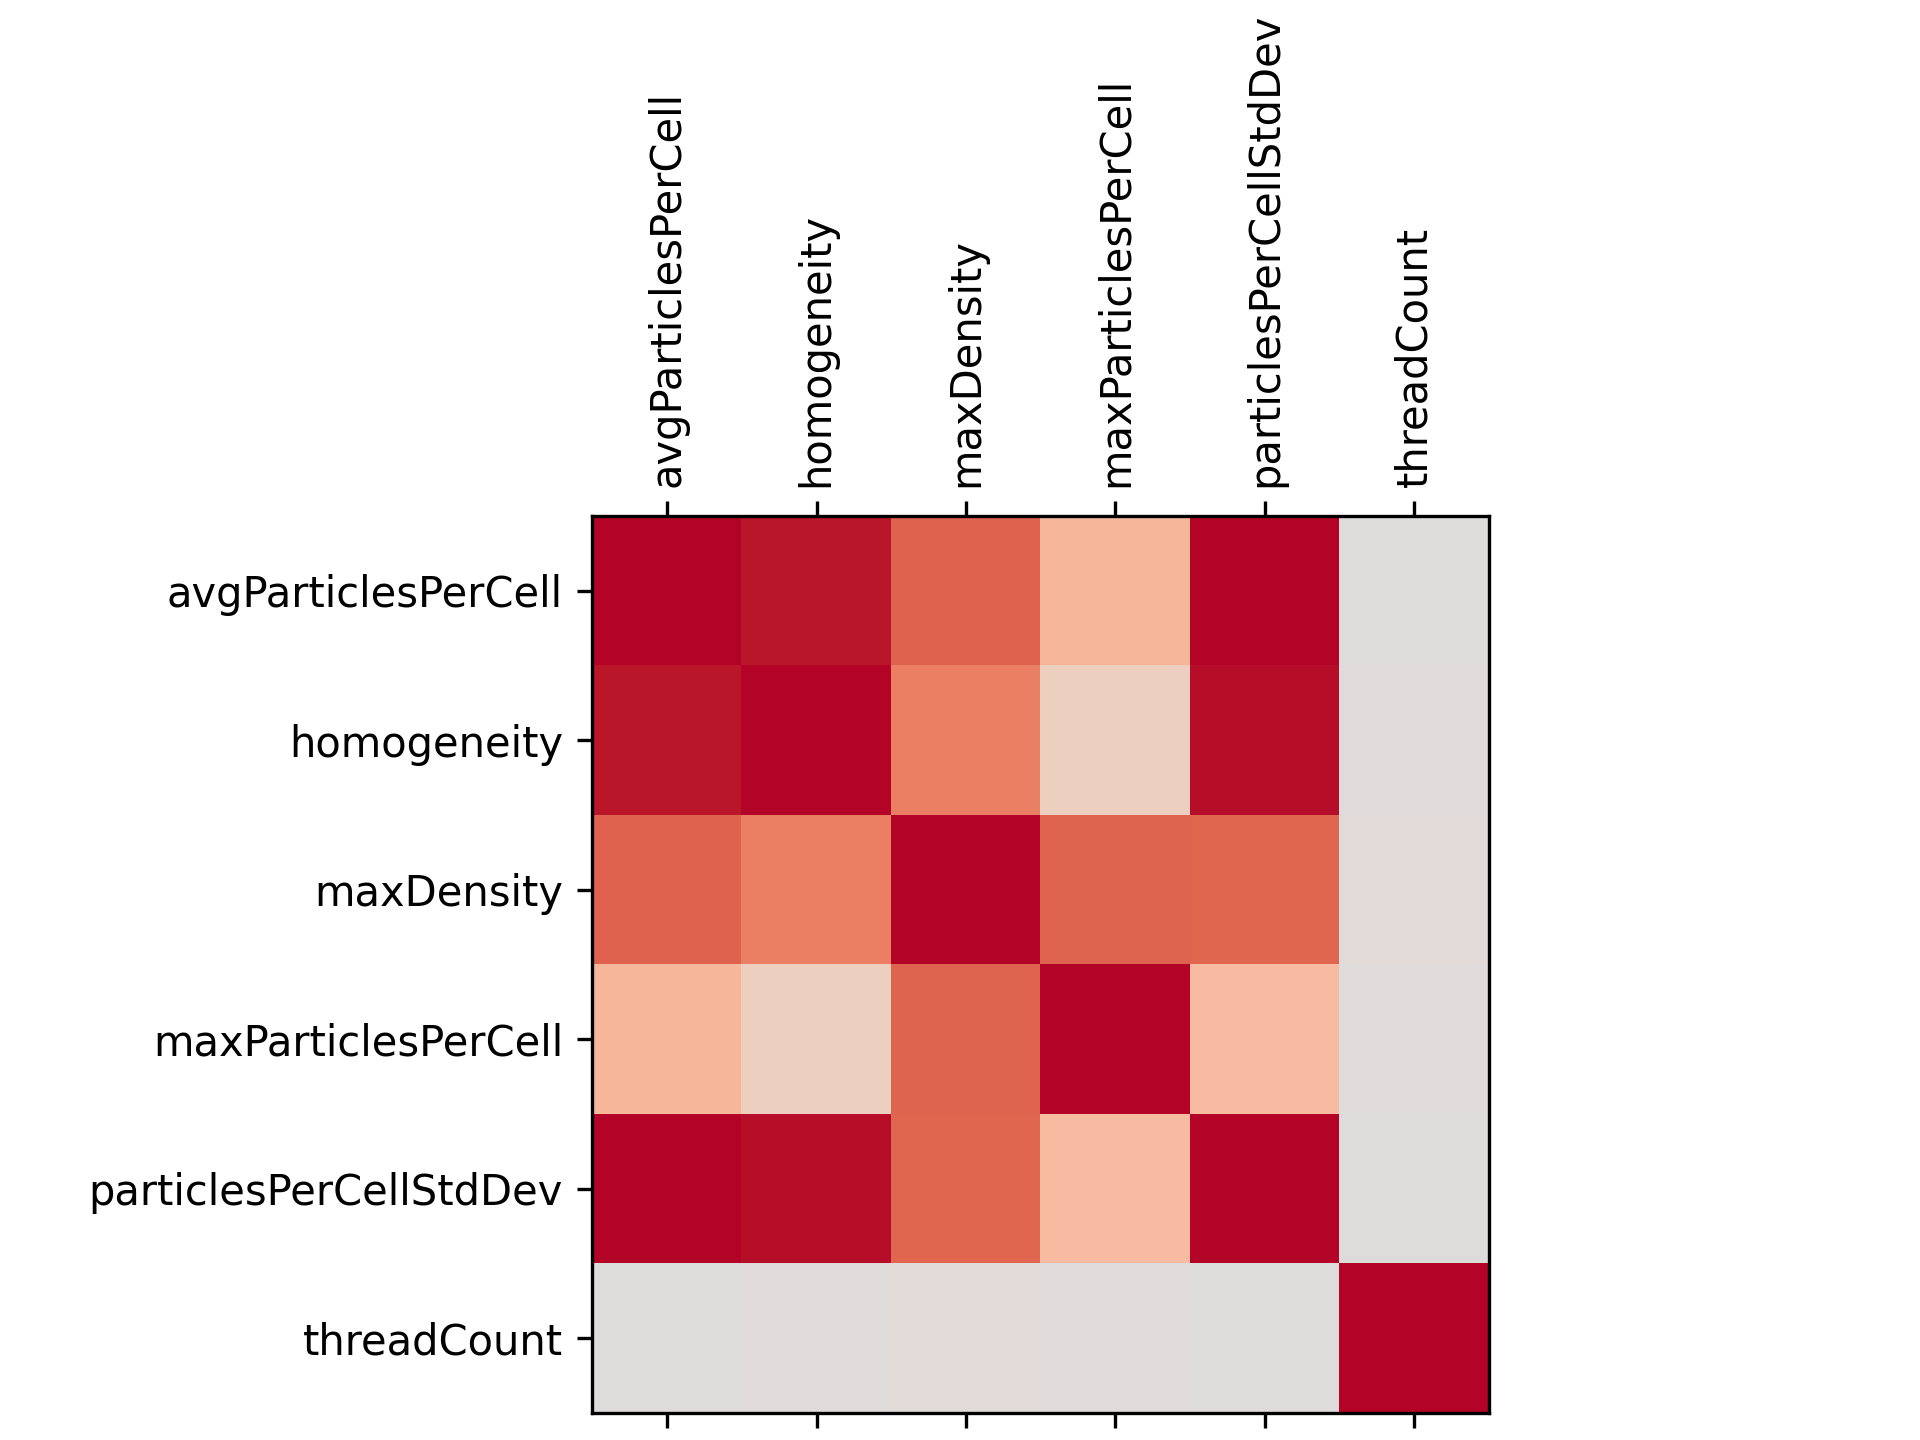
\includegraphics[height=5cm,trim={0cm 0 2cm 0cm},clip]{figures/DataAnalytics/correlation_matrix.png}
  \caption[Correlation Matrix of the collected Dataset]{Correlation matrix showing the correlation between the collected parameters of the LiveInfoData files. We can see that many of the collected parameters are slightly positively correlated with each other.}
  \label{fig:corrMatrix}
\end{figure}

\begin{figure}[H]
  \centering
  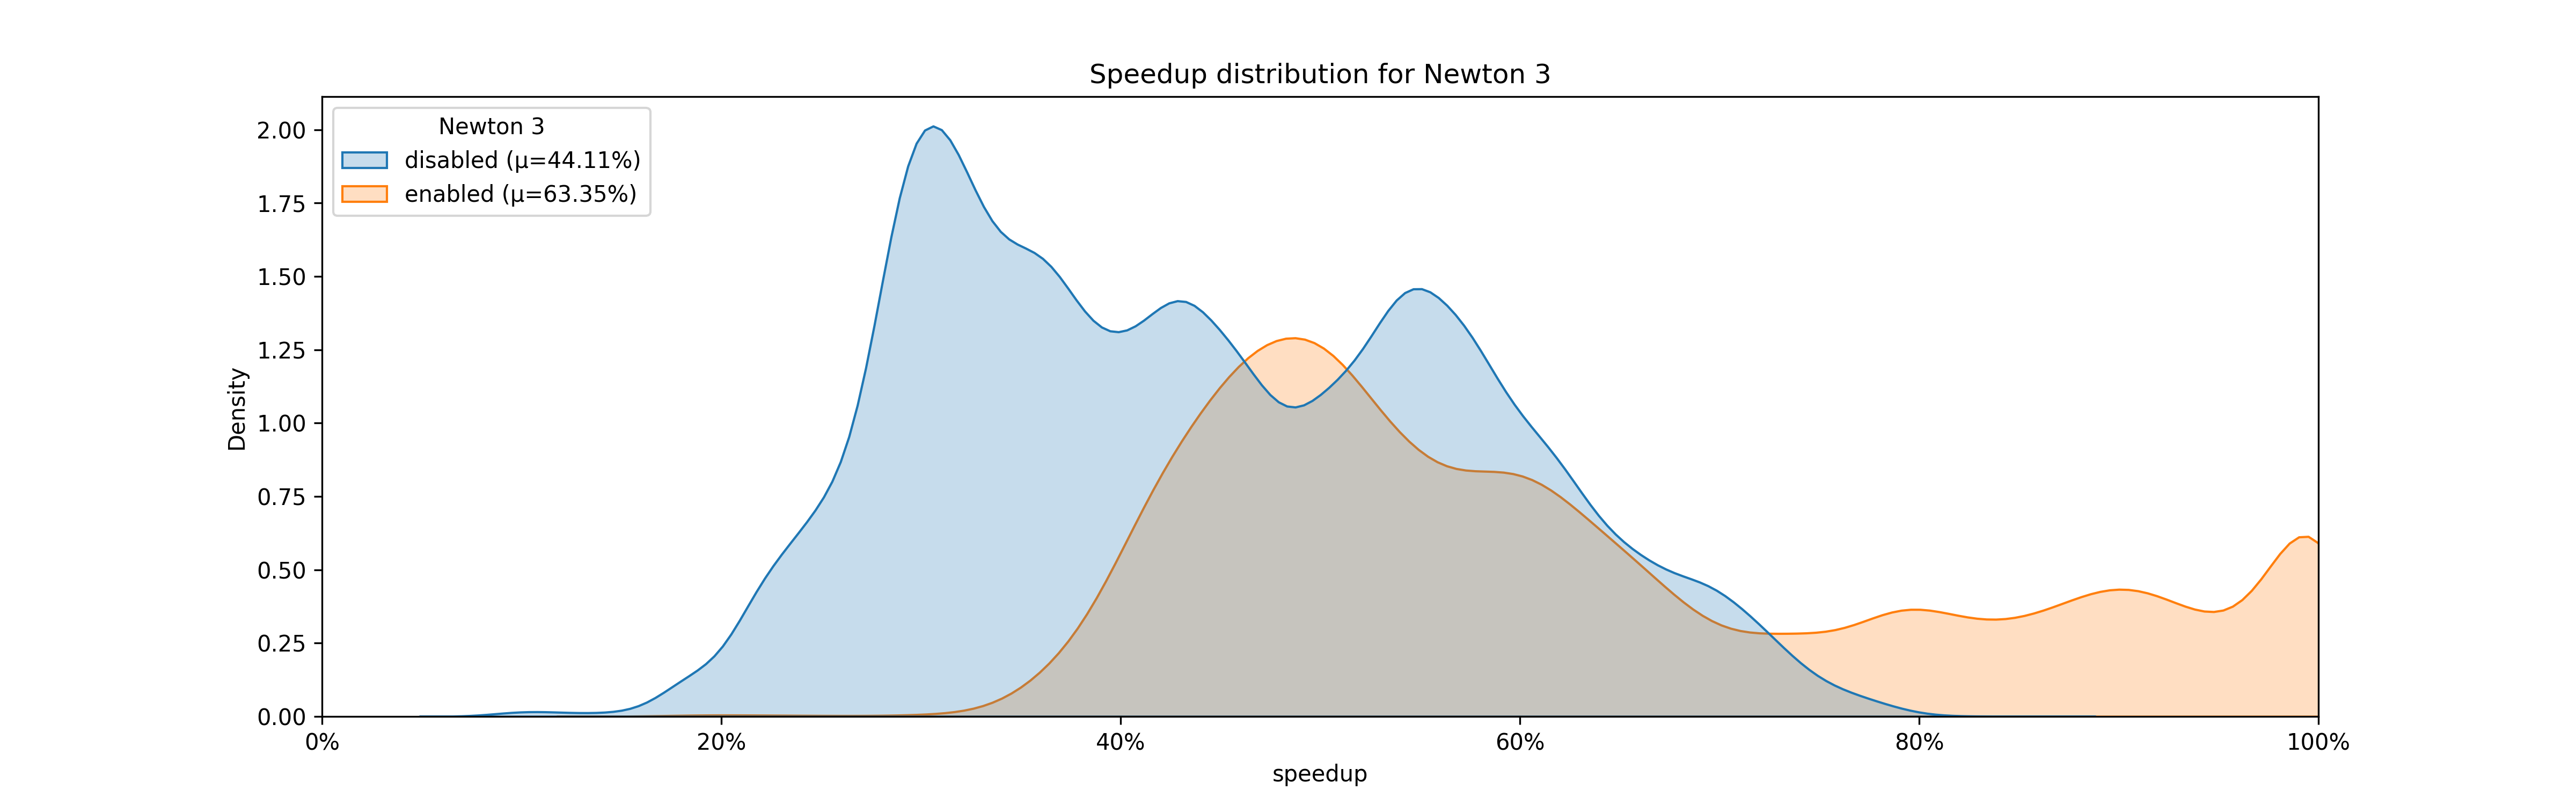
\includegraphics[width=\columnwidth,trim={1cm 0 2cm 1.5cm},clip]{figures/DataAnalytics/speedup_Newton 3.png}
  \caption[Speedup density plot based on the Newton 3 option]{Density plot showing the distribution of the relative speedup based on the Newton 3 option. We can see that Newton3=enabled is generally the better option as it generally allows for a higher relative speedup. All performances with relative speedups of at least 80\% use the Newton3 optimization. Therefore, we can confirm that Newton 3 is generally a good option.}
  \label{fig:inputAnalysisDensityNewton3}
\end{figure}

\begin{figure}[H]
  \centering
  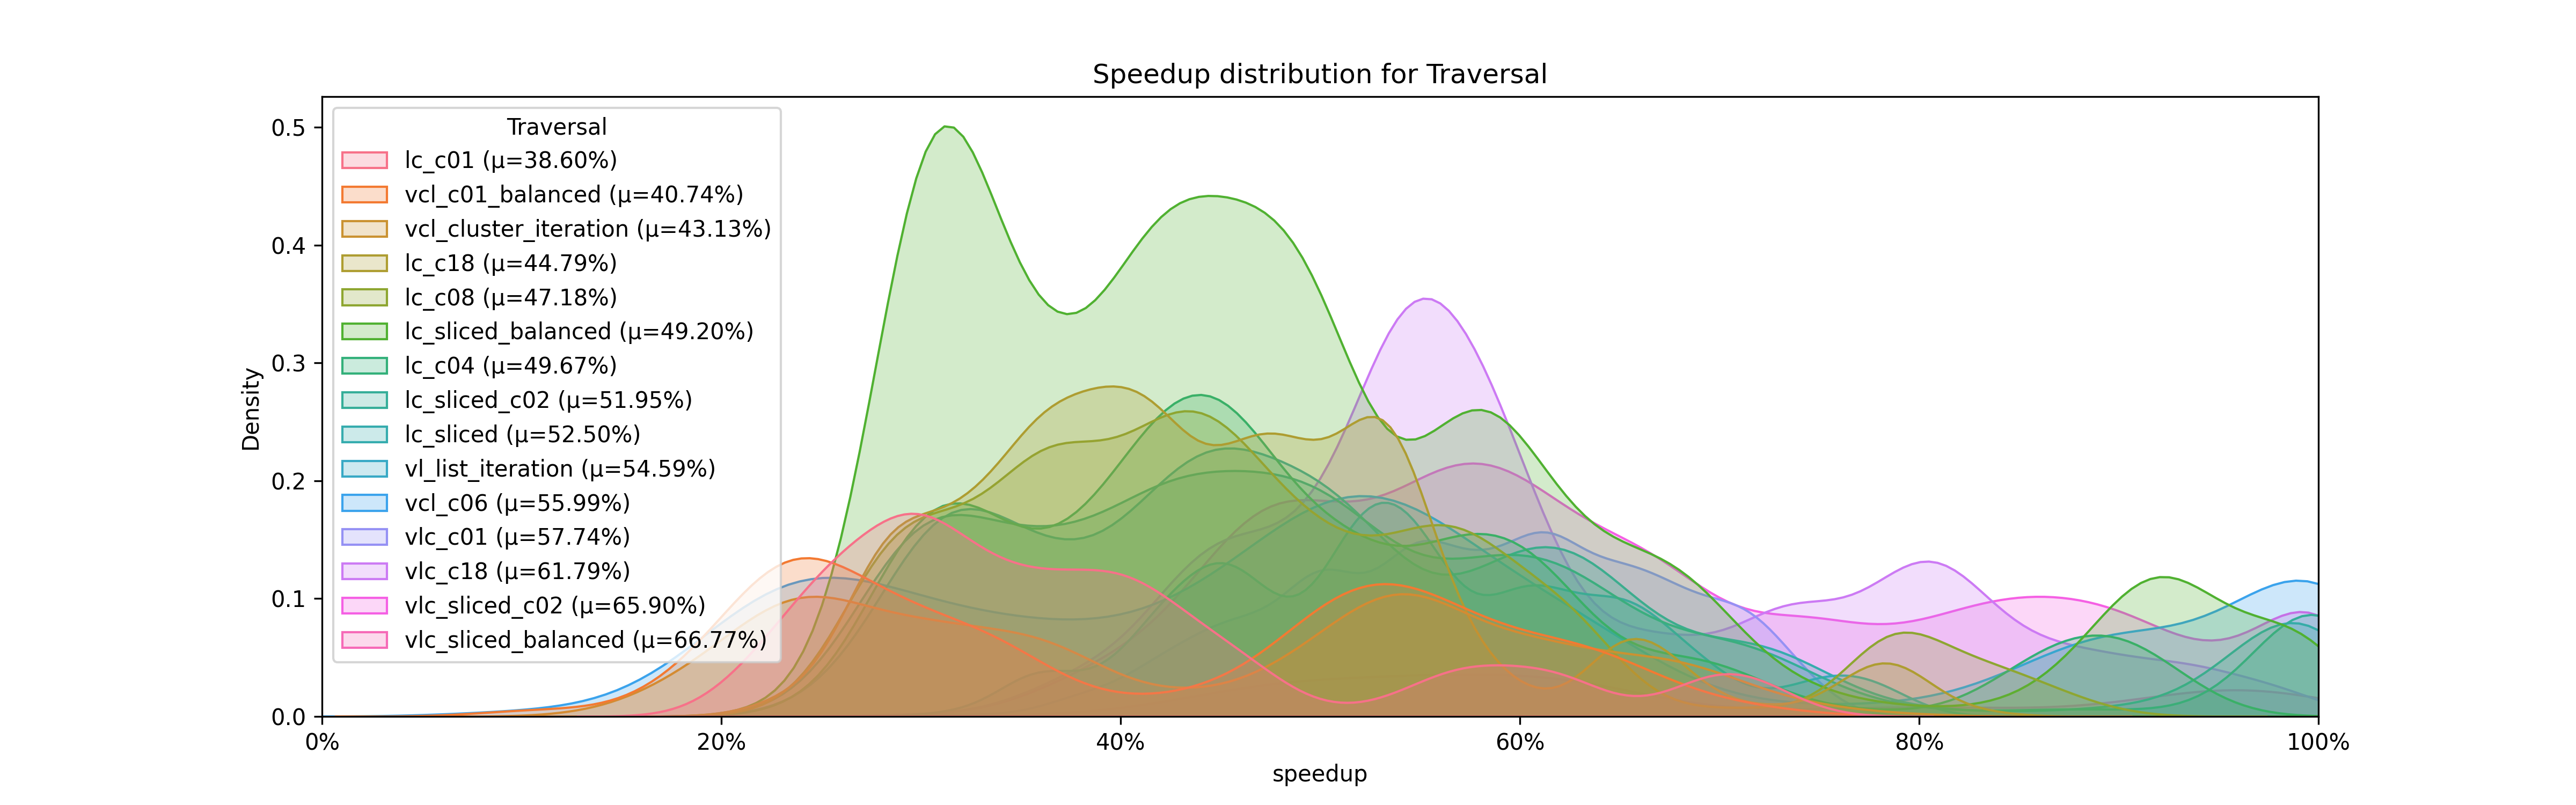
\includegraphics[width=\columnwidth,trim={1cm 0 2cm 1.5cm},clip]{figures/DataAnalytics/speedup_Traversal.png}
  \caption[Speedup density plot based on the Traversal option]{Density plot showing the distribution of the relative speedup based on the Traversal option. We can see that the vlc\_sliced\_balanced option generally performed better than the other options on this dataset with an expected relative speedup of 66\%.}
  \label{fig:inputAnalysisDensityTraversal}
\end{figure}

\begin{figure}[H]
  \centering
  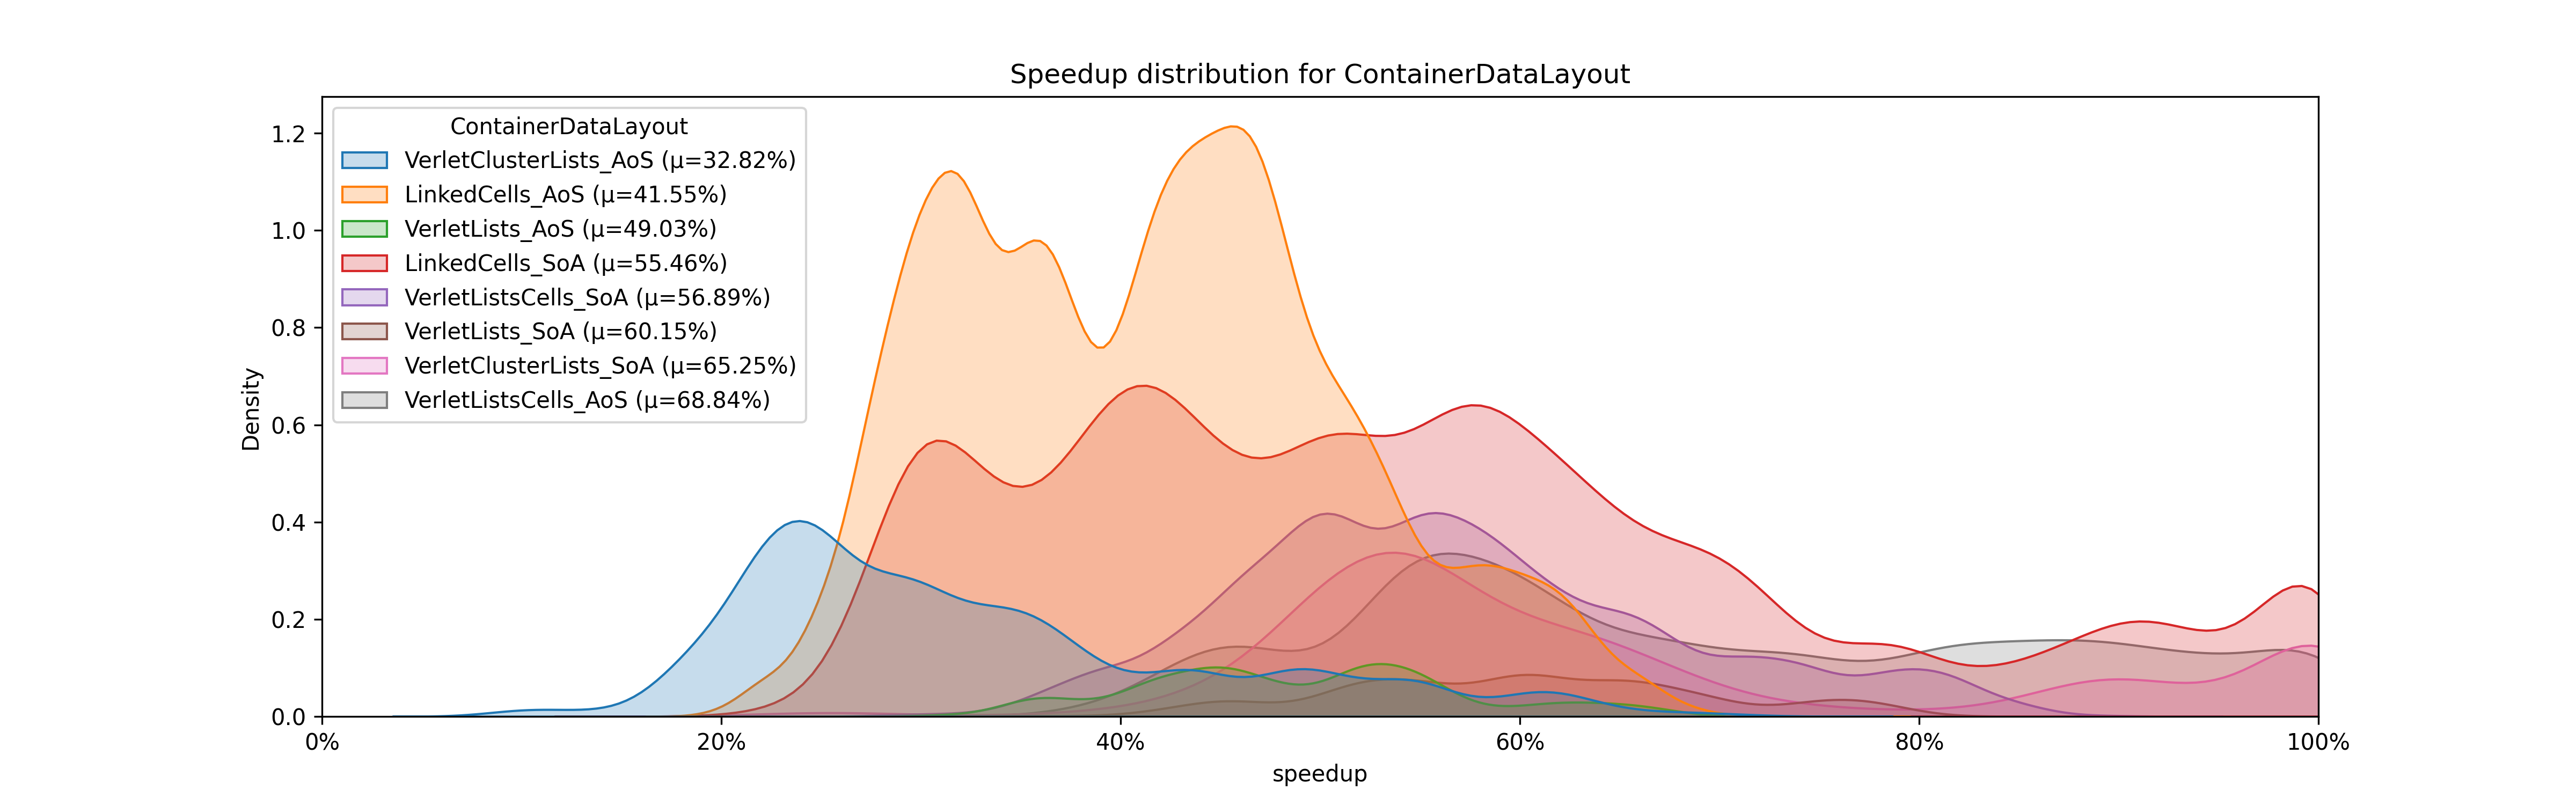
\includegraphics[width=\columnwidth,trim={1cm 0 2cm 1.5cm},clip]{figures/DataAnalytics/speedup_ContainerDataLayout.png}
  \caption[Speedup density plot of Configuration-Datalayout option]{Density plot showing the distribution of the relative speedup based on the ContainerDatalayout option. The VerletListCells\_AoS ContainerDatalayout performed best on this dataset with an expected relative speedup of 68.8\%.}
  \label{fig:inputAnalysisDensityDatalayout}
\end{figure}